
\section{NLLENS: Nonlinear Lens with Elliptic Potential}

\begin{verbatim}
label: NLLENS, KNLL = real, CNLL = real;
\end{verbatim}

The NLLENS element represents a thin nonlinear lens with the potential
of 'Elliptic' type as specified in [1]. The lens is used to create fully
integrable 2D nonlinear accelerator lattice with very large nonlinear
tune spread/shift. The NLLENS element is recognized by the thin tracking
module. The quadrupole term of the potential is included in the
TRANSPORT map and, consequently, effects the calculation of tunes and
Twiss functions.   

\begin{itemize}
   \item KNLL: The integrated strength of lens (m). The strength is
     parametrized so that     the quadrupole term of the multipole
     expansion is k1=2*KNLL/CNLL\textasciicircum2.      
   \item CNLL: The dimensional parameter of lens (m). The singularities
     of the potential are     located at X=-CNLL,+CNLL and Y=0.  
\end{itemize}

The scalar potential function of the element is given by
\\
%%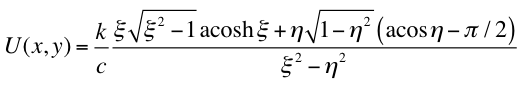
\includegraphics{nllens_potential.png}
%nllens_potential
\[
U(x,y)=\frac{k}{c}\frac{\xi\sqrt{\xi^2-1} \, \text{acosh}\xi + \eta\sqrt{1-\eta^2}(\text{acos}\eta-\pi/2)}{\xi^2-\eta^2}
\]
\\ where 
%%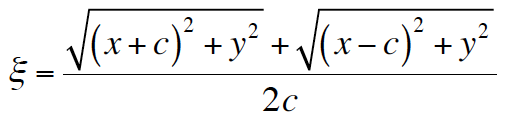
\includegraphics{nllens_xi.png}, 
%%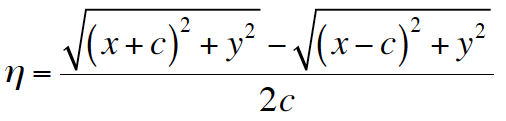
\includegraphics{nllens_eta.png}, and \textit{k} = KNLL, \textit{c} = CNLL. 
%nllens_xi
\[
\xi = \frac{\sqrt{(x+c)^2+y^2}+\sqrt{(x-c)^2+y^2}}{2c}, \quad \eta = \frac{\sqrt{(x+c)^2+y^2}-\sqrt{(x-c)^2+y^2}}{2c},
\]
and \textit{k} = KNLL, \textit{c} = CNLL.

Figure below shows the contour plot of the scalar potential: \\
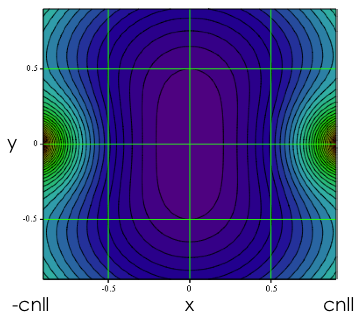
\includegraphics[width=220px]{Introduction/nllens_potential-2D.png}

The multipole expansion of the scalar potential is \\
%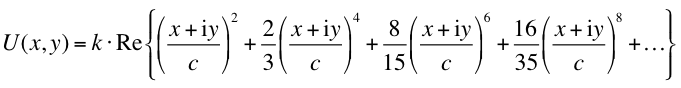
\includegraphics{Introduction/nllens_potential-expansion.png}
%nllens_potential-expansion
\[
U(x,y)=k\cdot Re\left\{ \left(\dfrac{x + i y}{c}\right)^2 + \frac{2}{3}\left(\dfrac{x + i y}{c}\right)^4 + \frac{8}{15}\left(\dfrac{x + i y}{c}\right)^6 + \frac{16}{35}\left(\dfrac{x + i y}{c}\right)^8 + \cdots \right\}
\]
\\ 
Note that this expansion is only valid inside the \textit{r=c} circle on
the x,y plane.    

In order to create integrable optics, one needs to shape the potential
along z axis according to the beta-function. Below is an example
nonlinear section representing the necessary nonlinear field with 20
thin lenses:  
\begin{verbatim}
    mu0 = 0.3;  ! phase advance over straight section
    l0 = 2.0;   ! length of the straight section
    nn = 20;    !number of nonlinear elements
    tn = 0.45;  ! strength of nonlinear lens
    cn = 0.01;  ! dimentional parameter of nonlinear lens

    musect = mu0 + 0.5;
    f0 = l0/4.0*(1.0+1.0/tan(pi*mu0)^2);
    betae = l0/sqrt(1.0-(1.0-l0/2.0/f0)^2);
    alfae = l0/2.0/f0/sqrt(1.0-(1.0-l0/2.0/f0)^2);
    betas = l0*(1-l0/4.0/f0)/sqrt(1.0-(1.0-l0/2.0/f0)^2);
    value, f0, betae, alfae, betas;

    ncreate(ii,kk,cc): macro = {n.ii: nllens, knll=kk, cnll=cc;};

i=0;
while(i <  nn)
  {
    i = i+1;
    sn = l0/nn*(i-0.5);
    bn = l0*(1-sn*(l0-sn)/l0/f0)/sqrt(1.0-(1.0-l0/2.0/f0)^2);
    knn = l0*tn*cn^2/nn/bn;
    cnn = cn*sqrt(bn);
    exec, ncreate($i,knn,cnn);
    value, i, bn, cnn, knn;
  };
\end{verbatim}

%% To be moved in References at the end of the document
References:
\begin{enumerate}
\item V. Danilov, S. Nagaitsev, Phys. Rev. ST Accel. Beams \textbf{13},
  084002 (2010). 
  
\item A. Valishev, S. Nagaitsev, V. Kashikhin, V. Danilov, in
  Proceedings of 2011 Particle Accelerator Conference, New York, NY,
  USA, WEP070. 
\end{enumerate}

%A. Valishev, March 19, 2012
